\documentclass{article}

% set font encoding for PDFLaTeX or XeLaTeX
\usepackage{ifxetex}
\ifxetex
  \usepackage{fontspec}
\else
  \usepackage[T1]{fontenc}
  \usepackage[utf8]{inputenc}
  \usepackage{lmodern}
  \usepackage{graphicx}
\fi

% used in maketitle
\usepackage[left=3cm,right=3cm,top=3cm,bottom=3cm]{geometry}
\title{Evaluación1}
\author{Luis Aarón Cerón Ramírez}

% Enable SageTeX to run SageMath code right inside this LaTeX file.
% documentation: http://mirrors.ctan.org/macros/latex/contrib/sagetex/sagetexpackage.pdf
% \usepackage{sagetex}

\begin{document}
\maketitle
La acticvidad consistio en hacer diferentes graficas con diferentes paquetes, de dos archivos diferentes los cuales provenian de mediciones tomadas en el manglar El Sargento, en una bahia en la costa frente a la parte norte de la Isla Tiburon.
\newline
Las variables atmosfericas medidas fueron CO2, radiación solar, nivel de agua y salinidad en el Manglar.
\newline
Se comenzo por revisar los documento: sargento\-201117.csv y  Salinidad: salinidad\_sargento-201117.csv, datos que fueron tomados en febrero del 2018 que fueron tomados con una frecuencia cada 15 minutos.
\newline
Se comenzo por capturar los datos de los dos archivos en jupyter notebook, una vez hecho esto se convirtio la variable fecha en meses para asi poder trabajar mas facilmente con los datos, este fue le codigo usado:
\begin{verbatim}
df['Ndate'] = pd.to_datetime(df['Date'], format = '%m/%d/%Y %H:%M:%S')
df['month'] = df['Ndate'].dt.month
df.head()
\end{verbatim}

Una vez hecho esto se realizaron los siguites diagramas de cajas:
\begin{verbatim}
import seaborn as sns
import matplotlib.pyplot as plt
plt.title("Diagrama de caja de date vs wate_level")
ax = sns.boxplot(x="month", y="water_level", data=df)
plt.show()
\end{verbatim}

\begin{figure}[h]
\centering
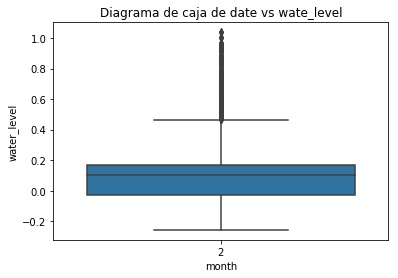
\includegraphics[scale=0.5]{diagrama1.png}
\caption{Diagrama de caja}
\end{figure}

\begin{verbatim}
import seaborn as sns
import matplotlib.pyplot as plt
plt.title("Diagrama de caja de date vs Temp")
ax = sns.boxplot(x="month", y="Temp", data=df)
plt.show()
\end{verbatim}

\begin{figure}[h]
\centering
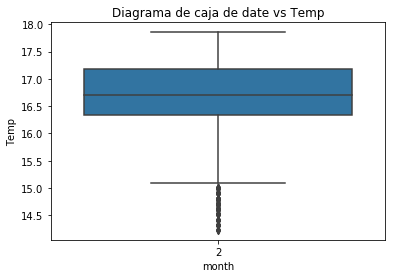
\includegraphics[scale=0.5]{diagrama2.png}
\caption{Diagrama de caja}
\end{figure}

Despues se pidio hacer unos diagrama de Pearson, para esto era necesario combinar los archivos, por lo que se utilizo la funcion concatenar para asi poder hacer los diagramas.
El fragmeto de codigo utilizado para esto es el siguiente:
\begin{verbatim}
df2 = pd.concat([df['water_level'], df1['salinity']], axis=1)
df2.head()
\end{verbatim}

Una vez hecho esto se pudo hacer el diagramade Pearson de water\_level vs salinity

\begin{figure}[h]
\centering
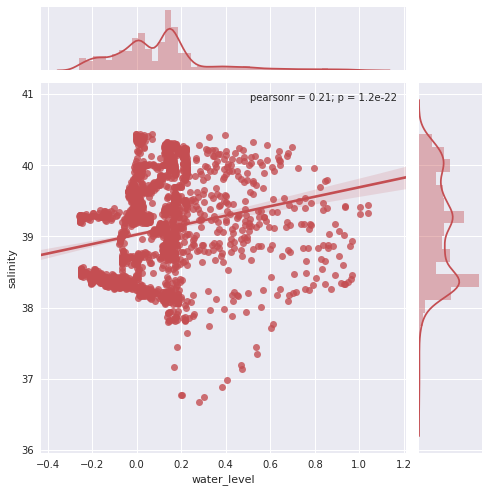
\includegraphics[scale=0.5]{pearson1.png}
\caption{Diagrama de Pearson}
\end{figure}


Se volvio a realizar el mismo procedimiento concatenado, ahora la variable temp y water\_level
Despues se hizo el  diagramade Pearson de water\_level vs temp
\begin{verbatim}
sns.set(style="darkgrid", color_codes=True)
g = sns.jointplot("water_level", "temp", data=df3, kind="reg", color="r", size=7)
plt.show(g)
\end{verbatim}

\begin{figure}[h]
\centering
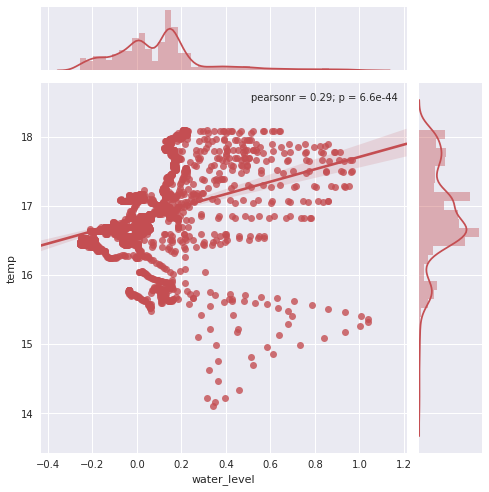
\includegraphics[scale=0.5]{pearson2.png}
\caption{Diagrama de Pearson}
\end{figure}

Para obtener el tercer grafico se hizo exactamente lo mismo, pero relacionando las columnas salinity vs temp
\begin{verbatim}
import seaborn as sns
sns.set(style="darkgrid", color_codes=True)
g = sns.jointplot("salinity","Temp",  data=df4, kind="reg", color="r", size=7)
plt.show(g)
\end{verbatim}

\begin{figure}[h]
\centering
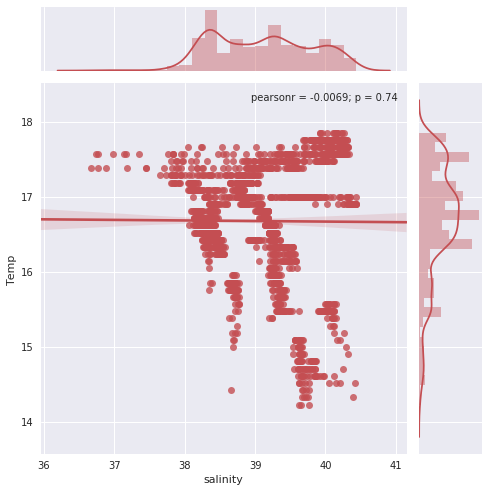
\includegraphics[scale=0.5]{pearson3.png}
\caption{Diagrama de Pearson}
\end{figure}


Despues se realizo una grafica de tiempo vs temp
\begin{verbatim}
plt.plot_date(x=df.Date, y=df.Temp, fmt="b-")
plt.title("Fecha vs nivel del mar ")
plt.ylabel("Temp ºC")
plt.xlabel("fecha")
plt.grid(True)
plt.show()
\end{verbatim}

\begin{figure}[h]
\centering
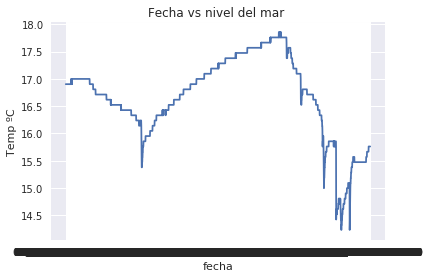
\includegraphics[scale]{fecha.png}
\caption{grafica de fecha vs temp}
\end{figure}

Despues de una de salinity vs water\_level
\begin{verbatim}
df2 = df2[['water_level','salinity']]
plt.figure(); df2.plot(); plt.legend(loc='best')
plt.title("")
plt.ylabel("water_level/(%) salinity")
plt.grid(True)
plt.show()
\end{verbatim}
y su grafica

\begin{figure}[h]
\centering
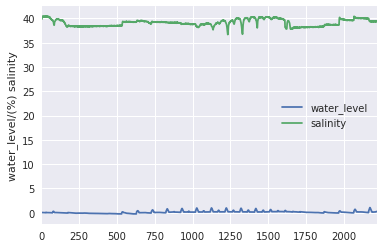
\includegraphics[scale=0.5]{dos.png}
\caption{Diagrama de Pearson}
\end{figure}

\end{document}
